 \documentclass{standalone}
 \usepackage[utf8]{inputenc}
 \usepackage{tikz}
 \begin{document}

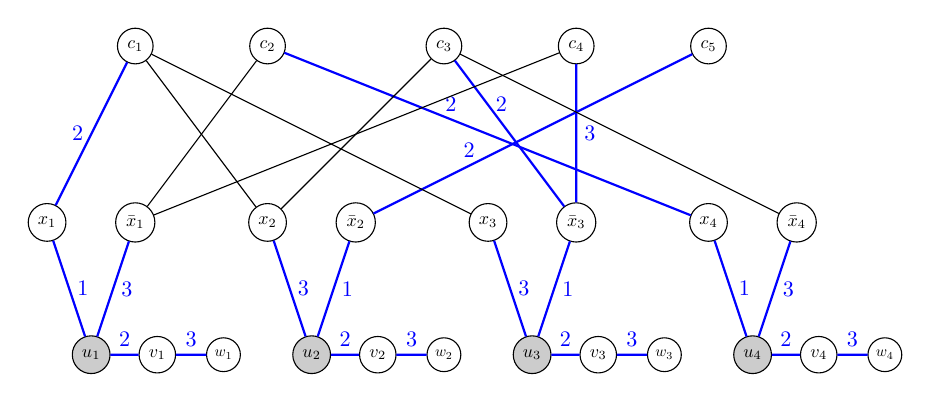
\begin{tikzpicture}[scale=.7] 
  \begin{scope}[scale=.8,auto=left,every node/.style={circle,fill=none,scale=.65,draw} ]
    %\node[fill=gray!40] (s1) at (0,3) {$s_1$}; 
    %\node[fill=gray!40] (s2) at (5,3) {$s_2$}; 
    %\node[fill=gray!40] (s3) at (10,3) {$s_3$}; 
    %\node[fill=gray!40] (s4) at (15,3) {$s_4$}; 
    \node[fill=gray!40] (ux1) at (0,5)  {$u_1$}; \node (vx1) at (1.5,5) {$v_1$};\node[scale=.85] (wx1) at (3,5) {$w_1$};
    \node[fill=gray!40] (ux2) at (5,5)  {$u_2$}; \node (vx2) at (6.5,5) {$v_2$};\node[scale=.85] (wx2) at (8,5) {$w_2$};
    \node[fill=gray!40] (ux3) at (10,5)  {$u_3$};\node (vx3) at (11.5,5) {$v_3$};\node[scale=.85] (wx3) at (13,5) {$w_3$};
    \node[fill=gray!40] (ux4) at (15,5)  {$u_4$};\node (vx4) at (16.5,5) {$v_4$};\node[scale=.85] (wx4) at (18,5) {$w_4$};
  
  \node (x11) at (-1,8)  {$x_1$};
    \node (x10) at (1,8)  {$\bar{x}_1$};
    \node (x21) at (4,8)  {$x_2$};
    \node (x20) at (6,8)  {$\bar{x}_2$};
    \node (x31) at (9,8) {$x_3$};
    \node (x30) at (11,8) {$\bar{x}_3$};
    \node (x41) at (14,8) {$x_4$};
    \node (x40) at (16,8) {$\bar{x}_4$};

    \node (c1) at (1,12)  {$c_1$};
    \node (c2) at (4,12)  {$c_2$};
    \node (c3) at (8,12)  {$c_3$};
    \node (c4) at (11,12) {$c_4$};
    \node (c5) at (14,12) {$c_5$};
    \end{scope}

\begin{scope}[every edge/.style={draw=black}]
  %\foreach \from\to in {s1/ux1,s2/ux2,s3/ux3,s4/ux4}
  %	\draw (\from) edge[blue,thick] node [right, midway,scale=.8] {1} (\to) ;
  \foreach \from\to in {ux1/x11,ux2/x20,ux3/x30,ux4/x41}
  	\draw (\from) edge[blue,thick,thick] node [right,midway,scale=.8]{1} (\to);
  \foreach \from\to in {ux1/x10,ux2/x21,ux3/x31,ux4/x40}
  	\draw (\from) edge[blue,thick,thick] node [right,midway,scale=.8]{3} (\to);
   \foreach \from\to\label in {ux1/vx1/2,ux2/vx2/2,ux3/vx3/2,ux4/vx4/2,vx1/wx1/3,vx2/wx2/3,vx3/wx3/3,vx4/wx4/3}
  	\draw (\from) edge[blue,thick] node [above, midway,scale=.8] {\label} (\to) ;
 
%  \foreach \from\to\label in {x11/c1/3,x20/c5/3,x30/c3/3,x30/c4/4,x41/c2/3}
%  	\draw (\from) edge[blue,thick,thick] node [above,midway,scale=.8]{\label} (\to);
  	
	\draw (x11) edge[blue,thick,thick] node [left,midway,scale=.8]{2} (c1);
	\draw (x20) edge[blue,thick,thick] node [above,midway,scale=.8,style={pos=.3}]{2} (c5);
	\draw (x30) edge[blue,thick,thick] node [right,midway,scale=.8,style={pos=.7}]{2} (c3);
	\draw (x30) edge[blue,thick,thick] node [right,midway,scale=.8]{3} (c4);
	\draw (x41) edge[blue,thick,thick] node [above,midway,scale=.8,style={pos=0.59}]{2} (c2);
  
  \foreach \from\to in {x10/c2,x10/c4,x21/c1,x21/c3,x31/c1,x40/c3}
  	\draw (\from) edge node{} (\to);

\end{scope}
\end{tikzpicture}
\end{document}
